%link do tworzenia tabeli https://tablesgenerator.com
%symbole matematyczne: https://oeis.org/wiki/List_of_LaTeX_mathematical_symbols
%narzedzia matematyczne: https://en.wikibooks.org/wiki/LaTeX/Mathematics
%krótkie podpowiedzi http://www.mif.pg.gda.pl/homepages/sylas/students/wdi/doc/latex-sciaga.html
\documentclass{article}  %typ dokumentu
\usepackage[utf8]{inputenc} %rodzaj czcionki
\usepackage{geometry} %poprawienie marginesów
\usepackage{polski} %polskie znaki
\usepackage{multirow} %tabela
\usepackage{graphicx} %tabela
\usepackage{float} %tabela
\usepackage{diagbox} % 2 dane w jednym prostokącie
\usepackage{amsmath} % Matma
%\usepackage{blindtext} %
%\usepackage{enumitem}
\usepackage{tikz} %rysowanie
\usepackage{fancyhdr} %headery i footery
%\usetikzlibrary{arrows}
\graphicspath{{pictures/}}
\geometry{margin=0.7in}
% \textbf{pogrubienie}  \textit{kursywa}    \underline{podkreślenie}    

\pagestyle{fancy}
\fancyhf{}
%--------------------------------------------------------------
\def\tytul{Narzędzia pomiarowe} %<<<Tutaj wpisz tytuł ćwiczenia
%--------------------------------------------------------------
\begin{document}

    \lhead{Miernictwo elektroniczne - \tytul}
    \cfoot{\thepage}
    \rhead{\thepage}

    \begin{table}[H]
        \centering
        \resizebox{\textwidth}{!}{
        \begin{tabular}{|c|c|c|}
        \hline

        \begin{tabular}[c]{@{}c@{}}Byczko Maciej\\Malek Jan\\Maziec Michał\end{tabular}&
        \begin{tabular}[c]{@{}c@{}}Prowadzący:\\ Mgr Inż. Monika Prucnal\end{tabular} &
        \begin{tabular}[c]{@{}c@{}}Numer ćwiczenia\\
        %----------------------------------------
            1 %<<<tutaj wpisz numer ćwiczenia
        %----------------------------------------
        \end{tabular} \\ \hline
        \begin{tabular}[c]{@{}c@{}}Grupa nr.\\
        %----------------------------------------
            1 %<<<tutaj wpisz numer grupy
        %----------------------------------------    
        \end{tabular} & \begin{tabular}[c]{@{}c@{}}Temat ćwiczenia:\\\tytul
        \end{tabular}&Ilość punktów: \\ \hline\begin{tabular}[c]{@{}c@{}}Tydzień Nieparzysty\\ Godzina 11:15-13:00\end{tabular}&\begin{tabular}[c]{@{}c@{}}Data wykonania ćwiczenia:\\
        %----------------------------------------
        16 marca 2020 %<<<tutaj wpisz datę
        %----------------------------------------
        \end{tabular} &\\ \hline\end{tabular}}
    \end{table}
    % \begin{comment}
    % w części teoretycznej należy zawrzeć tutaj krótki wstęp teoretyczny,spis przyrządów, opis przebiegu doświadczenia, najlepiej w punktach
    % oblicznoe dokładności pomiarowe w tabelach, zaokrąglony przedział wyników pomiaru w tabelach, wykorzystane wzory, przykładowe obliczenia
    % opisane rysunki,schematy pomiarowe, wnioski końcowe !!! UNIKAĆ PUSTYCH PRZESTRZENI!!!
    % \end{comment}
    \centering
    \section{Część teoretyczna i opisowa}
        \subsection{cel ćwiczenia}
            \begin{flushleft}
                Celem ćwiczenia jest poznanie i pomiar cech prądu stałego, jego napięcia, natężenia i rezystancji.\\
                Używając wykonanych pomiarów możemy poznać niepewności pomiarowe oraz potwierdzić działanie prawa Ohma.
            \end{flushleft}
        \subsection{Wstęp teoretyczny}

        \subsection{program poszczególnych pomiarów}
            \begin{enumerate}
                \item Pomiar analogowy napięcia
                \begin{enumerate}
                    \item
                \end{enumerate}
                \item Pomiar cyfrowy napięcia
                    \begin{enumerate}
                        \item
                    \end{enumerate}
                \item Wzorzec rezystancji
                    \begin{enumerate}
                        \item
                    \end{enumerate}
            \end{enumerate}
        \subsection{spis przyrządów}
            \begin{table}[H]
                \centering
                \begin{tabular}{|c|c|c|c|}
                \hline
                Nr.&Przyrząd             &  Model   & Klasa przyrządu    \\ \hline
                1. &Zasilasz             & TYP 5121 &   ---------        \\ \hline
                2. &Woltomierz analogowy &   LM-3   &      0.5           \\ \hline
                3. &Woltomierz cyfrowy   &  UT803   &   ---------        \\ \hline
                4. &Amperomierz analogowy&   LM-3   &      0.5           \\ \hline
                5. &Amperomierz cyfrowy  &  UT803   &   ---------        \\ \hline
                6. &omomierz             &  UT803   &   ---------        \\ \hline
                \end{tabular}
            \end{table}

        \subsection{przebieg ćwiczenia}
            \begin{itemize}
                \item 
                \item 
                \item 
                \item 
            \end{itemize}
        \subsection{wzory}
            $\Delta U = \pm \frac{kl \ast U_z}{100}$

    \section{Pomiary i obliczenia}
        \subsection{Doświadczenie 1}
            \subsubsection{Schemat pomiarowy}
                \begin{figure}[H]
                    \centering
                    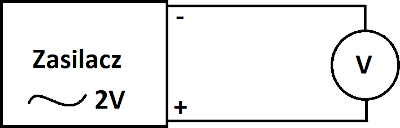
\includegraphics{zas-woltanal}
                    \caption{schemat pomiarowy}
                \end{figure}
            \subsubsection{Pomiary}
                \begin{table}[H]
                    \centering
                    \resizebox{\textwidth}{!}{
                    \begin{tabular}{|c|c|c|c|}
                    \hline
                    Nr. pomiaru & Zakres pomiaru{[}V{]} & Wskazania podziałki{[}max. 75 działek{]} & Wyniki pomiaru{[}V{]} \\ \hline
                    1. & 30  & 6  & 2.4  \\ \hline
                    2. & 15  & 11 & 2.2  \\ \hline
                    3. & 7.5 & 23 & 2.3  \\ \hline
                    4. & 3   & 58 & 2.32 \\ \hline
                    \end{tabular}}
                \end{table}
        \subsection{Obliczenia}
            Brak obliczeń
    \section{Wyniki i Wnioski}
    Pomiary są dosyć niedokładne z powodu analogowego sposobu dokonywania pomiarów
\end{document}
